A través de un visor de datos mantenido por NREL (National Renewable Energy
Laboratory), descargamos para el año 2022 un conjunto de valores climáticos con
frecuencia de 15 minutos. La información en si proviene del meteosat (figura
\ref{fig:meteosat_nsrdb}).

\begin{figure}[h] \centering
	\centering
	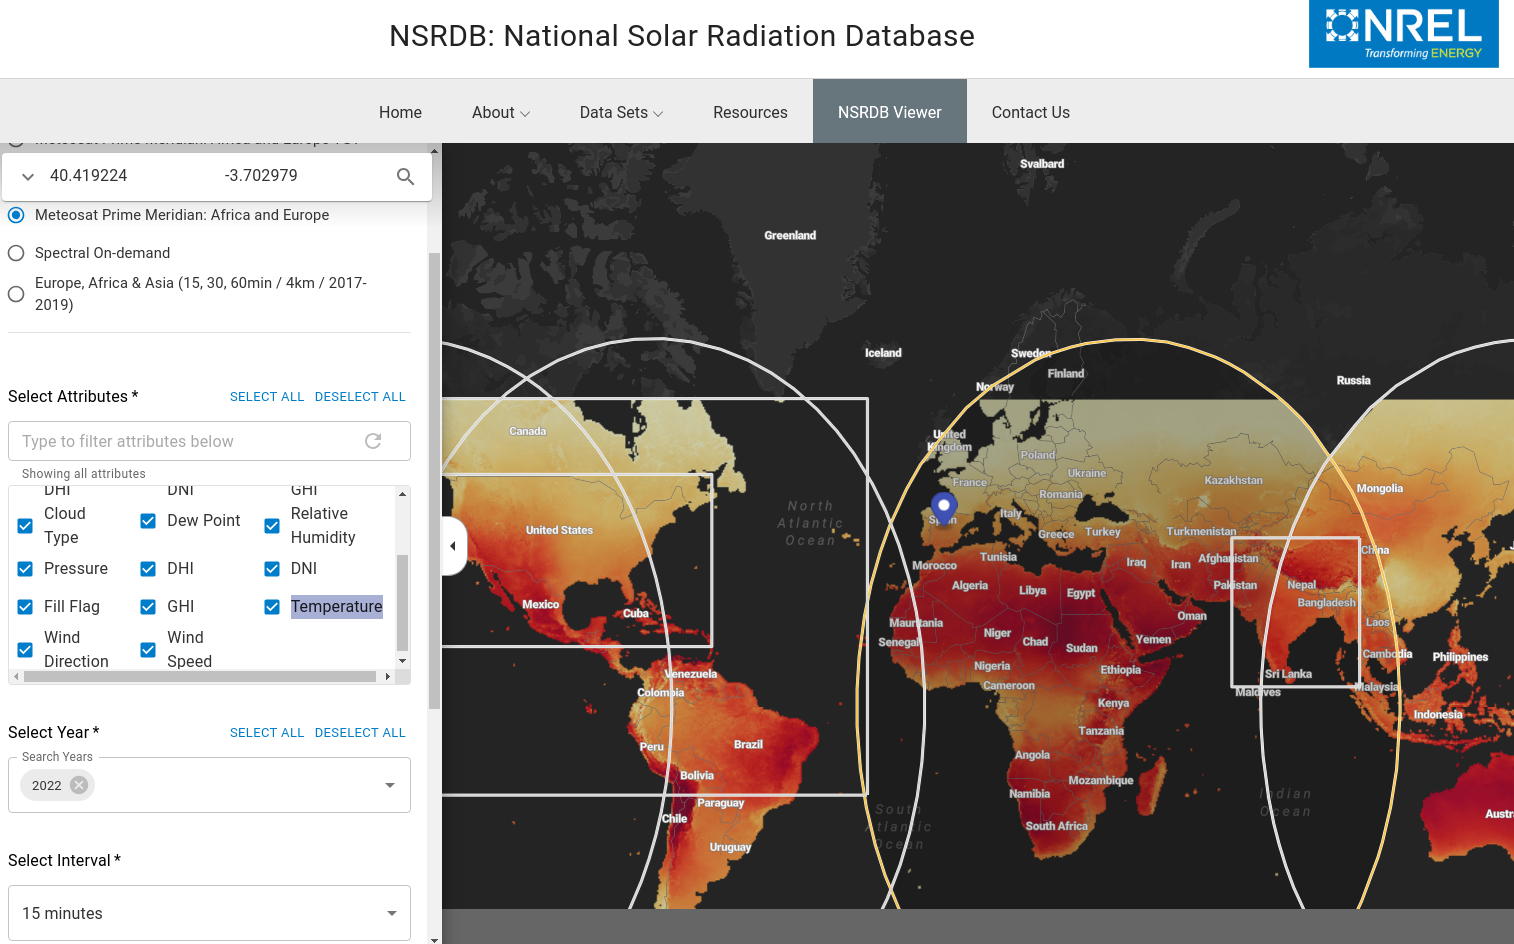
\includegraphics[width=1\textwidth]{./capitulos/adquisicion_de_datos/images/meteosat_nsrdb.png}
  \caption{Datos metereológicos del meteosat obtenidos a través de
  \url{https://nsrdb.nrel.gov/data-viewer}.}
	\label{fig:meteosat_nsrdb}
\end{figure}

Más notablemente, conseguimos las radiaciones solares globales (GHI: Global
Horizontal Irradiance, suma de la radiación directa y difusa), y las
temperaturas ambiente, que representamos en el gráfico
\ref{fig:temperatures_year}.

\begin{figure}[h] \centering
	\centering
	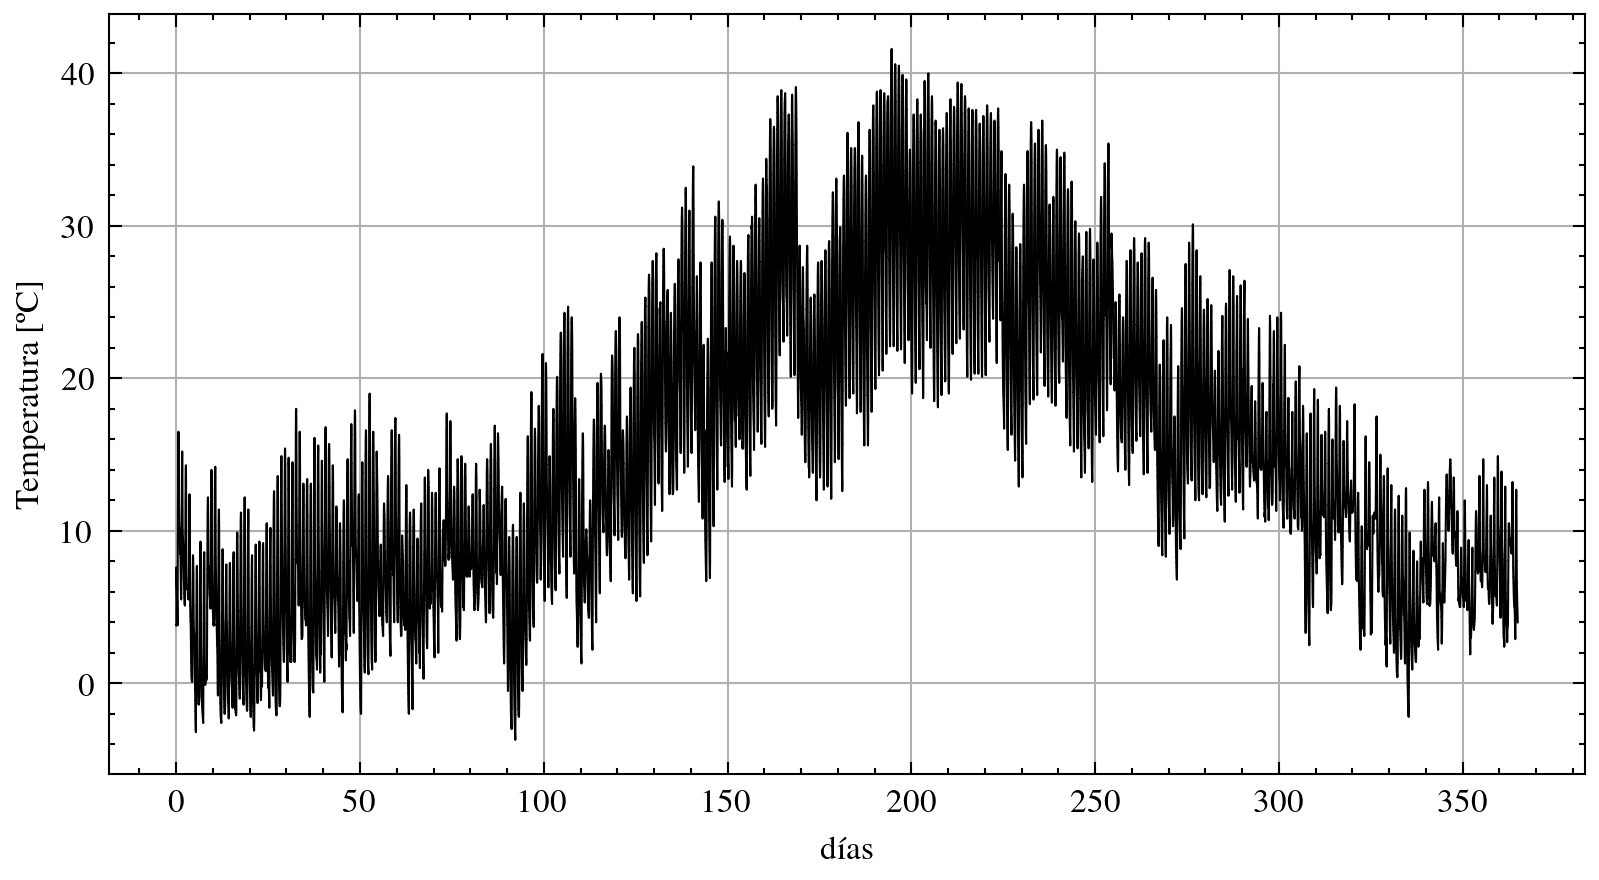
\includegraphics[width=1\textwidth]{./capitulos/adquisicion_de_datos/images/temperatures_year.png}
  \caption{Temperaturas para el año 2022 en Madrid.}
	\label{fig:temperatures_year}
\end{figure}
